\documentclass[12pt]{article}
\usepackage{graphicx}
\usepackage{amssymb}
\usepackage{listings}
\usepackage{amsmath}
\usepackage{graphicx}

% Russian specicfic
% -------------------------
\usepackage[T2A]{fontenc}
\usepackage[utf8]{inputenc}
\usepackage[russian]{babel}
% -------------------------

\begin{document}

\title{Общая связность сети. Критическое ребро.}

\author{
  Кирпа Вадим
  \and
  Махлярчук Андрей
  \and
  Утин Никита
  \and
  Березкин Аркадий
%  \and
%  Блинов Игорь
}

\maketitle
\thispagestyle{empty}
\newpage

\section{Постановка задачи:}

\paragraph{}
Для графа $G = (V, E, W)$ с множеством вершин $V$,
множеством ребер $W: E \rightarrow \mathbb{R}_+$
найти ребро $e^*$, такое, что при замене
$W(e^*) \rightarrow \gamma W(e^*)$ сумма сетевых 
расстояний между всеми узлами минимизируется
(при $\gamma < 1$) или максимизируется (при $\gamma > 1$).
Расчеты привести для графа Владивостока-2012.

\section{Алгоритм}

\paragraph{}
Для нахождения суммы сетевых расстояний в графе использовался
алгоритм Дейкстры\cite{dijkstra}.

\paragraph{}
Чтобы найти критическое ребро сумма сетевых расстояний считается
для всех подграфов $G_i$, где $W(e_i) \rightarrow \gamma W(e_i)$. Если сумма сетевых
ребер в текущем подграфе $G_i$ меньше (больше при $\gamma > 1$)
ранее найденой суммы, то это ребро сохраняется в качестве претендента
на критическое. В конце работы алгоритма мы получаем критическое ребро, 
сумму сетевых расстояний, соответствующую графу с обновленным весом критического ребра и новый вес данного ребра.

\section{Реализация} 
В начале выполнения программы происходит считывание графа из файла. 
Затем для каждой вершины запускаем алгоритм Дейкстры. В данной рализации можно было бы использовать 
алгоритм Флойда-Уоршелла, но было принято решение реализовать алгоритм Дейкстры, так как он легче поддается распараллеливанию.

\paragraph{}
Алгоритм реализован на языке C++. Основной процедурой является
алгоритм Дейкстры\cite{dijkstra}.

% \newpage

\begin{lstlisting}[language=C++]
void Graph::Dijkstra(int v) {
    std::vector<bool> visited(edges.size(), false);
    dists[v][v] = 0.0;
    std::priority_queue<
      std::pair<double, int>,
      std::vector<std::pair<double, int>>, Compare> q;
    visited[v] = true;
    q.push(std::make_pair(dists[v][v], v));

    while (!q.empty()) {
        std::pair<double, int> from = q.top();
        q.pop();
        for (auto& edge : edges[from.second]) {
            int to = edge.GetRight();
            if (!visited[to]) {
                double tmp = from.first + edge.GetWeight();
                if (dists[v][to] > tmp) {
                    dists[v][to] = tmp;
                    visited[to] = false;
                    q.push(std::make_pair(dists[v][to], to));
                }
            }
        }
    }
}
\end{lstlisting}

\paragraph{Оцена вычислительной сложности алгоритма.}

На данном графе $G = (V, E, W)$, алгоритм Дейкстры имеет вычислительную  сложность $O(V \log V + E) $.
В нашем алгоритме на каждое изменение веса ребра, запускается алгоритм Дейкстры из каждой вершины. В результате получаем 
вычислительную сложность алгоритма $O((V \log V + E)VE)$

\paragraph{Оптимизации:}
Чтобы ускорить исполнение программы, из каждой
вершины алгоритм Дейкстры запускается в отдельном
потоке. Т.к. граф разрежен в памяти он хранится в
виде списка смежности.

\section{Результаты}

\paragraph{Простой пример}

\paragraph{}

Рассмотрим простой пример работы алгоритма на графе с 6-ю вершинами и 5-ю ребрами
представленного на рис.~\ref{fig:min_graph_4} В данном случае мы будем минимизировать сумму сетевых расстояний и
примем $\gamma = 0.5$.

\begin{figure}[h]
    \centering
    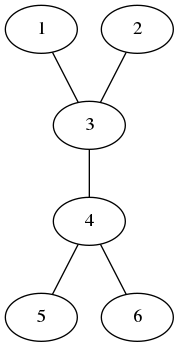
\includegraphics[scale=0.7]{min_graph_4.png}
    \caption{Малый граф с критическим ребром между 3-й и 4-й вершинами.}
    \label{fig:min_graph_4}
\end{figure}

Из каждой вершины исходного графа запустим алгоритм Дейкстры.
На каждом шаге работы алгоритма изменяем вес текущего ребра $W(e_i) \rightarrow \gamma W(e_i)$
Затем для данной итерации пересчитаем сумму сетевых расстояний, и, если она меньше текущей минимальной суммы,
то обновим минимум. Так в процессе работы алгоритма мы переберем все ребра и в качестве критического выберем 
ребро с соответствующей минимальной суммой сетевых расстояний. 
На каждой итерации работы алгоритма Дейкстры получим сумму сетевых расстояний для исходного графа:
\begin{gather}
1 : 1 + 5 + 6 + 6 + 2 \\
2 : 1 + 5 + 6 + 6 + 2 \\
3 : 1 + 1 + 4 + 5 + 5 \\
4 : 1 + 1 + 4 + 5 + 5 \\
5 : 1 + 5 + 6 + 6 + 2 \\
6 : 1 + 5 + 6 + 6 + 2
\end{gather}
Сумма сетевых расстояний в исходном графе $S = 112$. 

\begin{figure}[h]
    \centering
    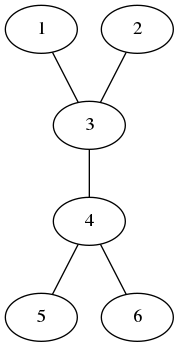
\includegraphics[scale=0.7]{min_graph_2.png}
    \caption{Если уменьшить вес ребра между 3-й и 4-й вершинами сумма сетевых расстояний минимизируется}
    \label{fig:min_graph_2}
\end{figure}

В данном граффе критическим является ребро между
3й и 4й вершинами и умножение его веса на
$\gamma < 1$ приводит к минимизации суммы сетевых расстояний.
При $\gamma = 0.5$ алгоритм меняет вес критического ребра на $0.5 \cdot W_i$ (рис.~\ref{fig:min_graph_2}).
Для обновленного графа, в котором мы заменили вес критического ребра на 2 получим сумму сетевых расстояний:
\begin{gather}
1 : 1 + 3 + 4 + 4 + 2 \\
2 : 1 + 3 + 4 + 4 + 2 \\
3 : 1 + 1 + 2 + 3 + 3 \\
4 : 1 + 1 + 2 + 3 + 3 \\
5 : 1 + 3 + 4 + 4 + 2 \\
6 : 1 + 3 + 4 + 4 + 2
\end{gather}
В таком случае сумма сетевых расстояний для обновленного графа будет равнятся $S^* = 76$.

\begin{figure}[h]
    \centering
    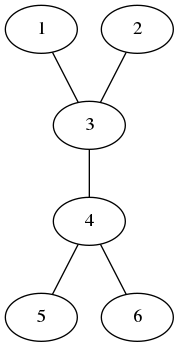
\includegraphics[scale=0.7]{min_graph_8.png}
    \caption{Если увеличить вес ребра между 3-й и 4-й вершинами сумма сетевых расстояний максимизируется}
    \label{fig:min_graph_8}
\end{figure}

\paragraph{Пример с графом срднего размера}

\section{Заключение}
Окончательное и обжалованию не подлежит

\begin{thebibliography}{9}
\bibitem{dijkstra}
Dijkstra E. W. \textit{A note on two problems in connexion with graphs} //
\textit{Numer. Math} — Springer Science+Business Media, 1959.
— Vol. 1, Iss. 1. — P. 269–271.
\end{thebibliography}

\end{document}
